\documentclass[letterpaper, 11pt]{article} 
\usepackage{fullpage} % changes the margin
\usepackage[english]{babel}
\usepackage[utf8]{inputenc}
\usepackage{amsmath}
\usepackage{graphicx}
\usepackage[colorinlistoftodos]{todonotes}
\usepackage{array}
\usepackage{longtable}

\begin{document}
%Header-Make sure you update this information!!!!
\noindent
\large\textbf{TinUg-Yu Wang, Duong Bui} \hfill \textbf{EE-393 Technical Writing} \\
\normalsize Quiz Section: AD \hfill Professor Bade \\
Date: 04/27/2016 \hfill TA: Julianne Dorothy Peeling \\

\section*{\centering{Solar Farm}}

\section*{Problem Statement}
Lack of electricity supply in rural areas.

\section*{Solution}
Utilizing vast flat lands in the rural area as a place to install solar farms. This helps generate extra electricity for both the rural and urban areas.

\section*{Product Specifications (Visuals)}
\begin{center}
    \begin{tabular}{| l | l |}
    \hline
    Size & 77" x 39" x 1.8"  \\ \hline
    Weight & 50 lb  \\ \hline
    Power Rating & 300 W \\ \hline
    Cost & \$200 / panel \\ \hline
    \end{tabular}
    \linebreak\linebreak Table 1: The AltE Photonic Solar Panel Specification
    
    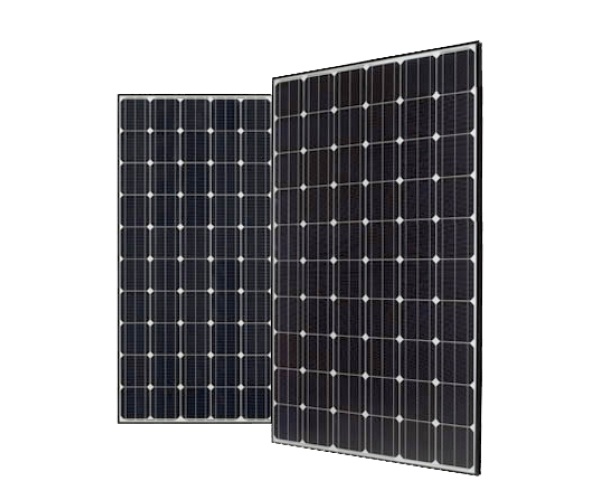
\includegraphics[scale=0.3]{solar}
    
    Figure 1: The AltE Photonic Solar Panel
    
\end{center}

\section*{Conclusion}
Solar power is consider to be unlimited source of green power as the Sun still be there in 4 or 5 billion more years. The initial cost maybe a huge amount but it’s a sustainable energy source for African people for decades.

\end{document}
